\section{Methods}\label{sec:methods}
% Model and analysis names introduced here are used unchanged in Results and Discussion.

\subsection{Study design}\label{sec:design}
This study used two public cohorts: NSCLC-Radiomics (LUNG1) for model development and internal evaluation, and NSCLC-Radiogenomics for external evaluation.\cite{tciaLung1,tciaRadiogenomics,bakr2018}
% Study design and analysis workflow. Included from sections/methods.tex (Study design).
% Source: figures/figure1/study_overview_fig.tex (build commands in its header).
\begin{figure}[!t]
\centering
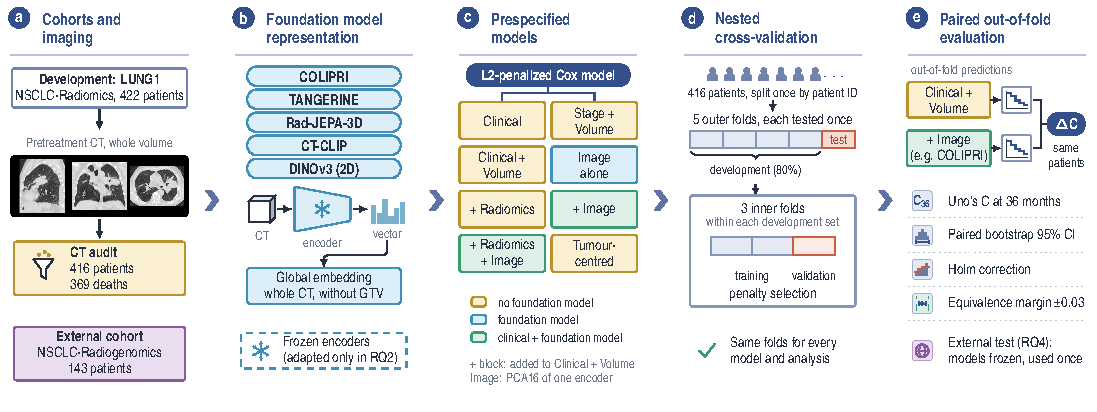
\includegraphics[width=\linewidth]{figures/study_overview.pdf}
\caption{Study design and analysis workflow. (a) LUNG1 provided all development data: after the CT audit, 416 patients had a pretreatment CT, a primary-tumour segmentation (GTV) and overall survival. NSCLC-Radiogenomics was used only for external evaluation. (b) Five foundation models encoded the whole CT with their published preprocessing and without the GTV into one global embedding per patient; the encoders were frozen except in the RQ2 adaptation analyses. (c) The prespecified models: nested clinical models, each adding one block to \model{Clinical+Volume}, the parsimonious \model{Stage+Volume} comparator, each image representation alone and the tumour-centred comparators. In the frozen benchmark, each embedding was reduced to its first 16 principal components (PCA16; 32, PCA32, in a sensitivity analysis), which entered an L2-penalized Cox model. (d) Five outer folds, fixed by patient before any model was fitted, and three inner folds for penalty selection were shared by every model and analysis. (e) Models were compared in pairs on the same test patients, for example \model{Clinical+Volume} with and without COLIPRI, by Uno's C at 36 months with paired bootstrap intervals, Holm correction and equivalence testing. For RQ4, models refitted on all 416 LUNG1 patients were frozen and applied once to the external cohort (purple).}
\label{fig:overview}
\end{figure}

The study was designed so that the main comparisons differ in the predictor being evaluated, while the evaluation protocol is held fixed. Every model, whether based on a whole-volume encoder, on tumour-centred features or on clinical covariates alone, was evaluated on the same patients, the same five outer folds, the same endpoint and horizon and the same metric, so that every comparison is paired at the patient level. Each foundation model was used with its published preprocessing and pooling (Section~\ref{sec:representations}). The clinical models were not treated as one more representation but as the reference against which the added value of each image representation was assessed (Section~\ref{sec:clinical}). In the frozen benchmark, the five foundations also shared the same head (Section~\ref{sec:partitioning}), so that differences between them reflect the representation together with its preprocessing and pooling. Within this fixed design, the four research questions RQ1-RQ4 in Section~\ref{sec:intro} differ in what they vary:
\begin{itemize}
\item RQ1 compares the representations under one frozen head, and asks whether an image representation adds to clinical information through a nested sequence of clinical models.
\item RQ2 changes what is trained, from a more flexible head to the encoder itself, and how many patients are available for training.
\item RQ3 changes what the encoder can see, by pooling tokens from different regions and by hiding the tumour inside the encoder, and asks which clinical variables the embeddings encode.
\item RQ4 changes the population: models developed on all LUNG1 patients were frozen and applied once to the external cohort.
\end{itemize}
Figure~\ref{fig:overview} gives an overview of the study as a single workflow shared by all four questions. Table~\ref{tab:design} lists the primary and sensitivity analyses that address each question within this workflow.

\tabDesign

The remainder of this section first describes the elements shared by all analyses: the cohorts and endpoint (Section~\ref{sec:cohorts}), the image representations and tumour-centred comparators (Section~\ref{sec:representations}), the clinical reference models (Section~\ref{sec:clinical}), and the data partitioning, model selection and frozen head (Section~\ref{sec:partitioning}). It then details the analyses for each research question (Section~\ref{sec:analyses}) and the performance measures and statistical methods (Section~\ref{sec:stats}).

\subsection{Cohorts}\label{sec:cohorts}
Cohorts used in this study are public collections of The Cancer Imaging Archive and provide, for each patient, a pretreatment CT, a primary-tumour segmentation and overall survival, so that every model can be computed on the same patients. LUNG1 was used for model development and internal evaluation, and NSCLC-Radiogenomics only for external evaluation. For each cohort, we describe why it was chosen and how the patients analysed were selected. We then compare the characteristics of the two cohorts and their implications for the analyses.

\paragraph{Development cohort.} LUNG1 contains pretreatment planning CT, a delineated primary gross tumour volume (GTV) and overall survival for 422 patients with NSCLC treated with radiotherapy, with or without chemotherapy, at a single institution.\cite{aerts2014,tciaLung1} It was chosen for three reasons. It is one of the largest public CT cohorts with survival outcomes and the cohort on which radiomic and deep prognostic models were first developed,\cite{aerts2014,hosny2018} so our results can be placed against published work. It provides the tumour segmentation required by the tumour-centred comparators and by the tumour-perturbation analyses. Finally, its follow-up is almost complete within the evaluation horizon, which keeps the concordance estimates close to what would be observed without censoring.

Survival in LUNG1 is measured from the start of treatment; death is the event, and patients without a recorded death are right-censored. The cohort was audited before any model was run. Clinical and imaging records were joined by patient identifier, and we required a positive survival time, a valid event code and a complete CT series with consistent geometry (no duplicated slice positions and no interslice gap larger than 1.5 times the median). Five of the 422 patients failed the CT audit, and one further patient had no primary-tumour segmentation, leaving 416 patients with 369 deaths (Figure~\ref{fig:overview}). All internal analyses used these 416 patients, so whole-volume and tumour-centred models were always compared on identical patients. Missing clinical covariates did not exclude a patient.

\paragraph{External cohort.} NSCLC-Radiogenomics includes 211 patients with NSCLC from two institutions in the United States, most of them treated with surgical resection, with preoperative CT, clinical data and, for 144 of them, a tumour segmentation.\cite{bakr2018,tciaRadiogenomics} It was chosen because it is one of the few public cohorts that combine CT, overall survival and tumour segmentations from institutions other than the LUNG1 provider, so that the same models, including the tumour-centred ones, can be applied without modification. We used only the patients with a segmentation, so that every model could be computed on the same patients and every external comparison is paired. The protocol for the external evaluation was fixed before any image of this cohort was processed. Survival was measured from the date of the CT used as input, because treatment dates were not available. Because a patient can have several CT series, for example reconstructions with different slice thickness, we used the series on which the segmentation had been drawn, so that image and mask were aligned. The same CT audit as in LUNG1 excluded one patient with missing slices, leaving 143 patients. Because the segmentations in the source collection carry inconsistent labels (``Heart'', ``Tissue'', ``Segmentation''), we confirmed that each one marked the tumour: its centre had to lie within 1 mm of an independent tumour seed point\cite{pai2024} and the mask had to overlap the lung field.

\paragraph{Cohort characteristics and their implications.} Table~\ref{tab:cohorts} and Figure~\ref{fig:km} describe the cohorts. They differ in almost every respect that affects a survival model, and these differences determine how the results should be read.

\begin{figure}[!htbp]
\centering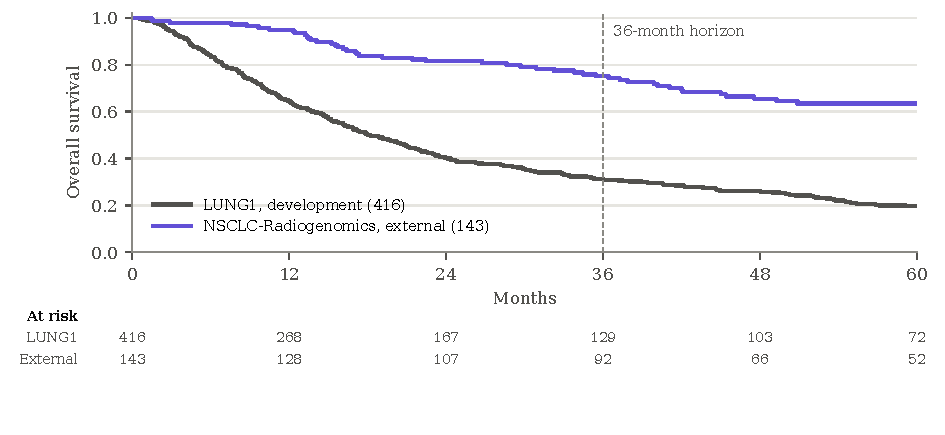
\includegraphics[width=\linewidth]{figures/cohort_km.pdf}
\caption{Kaplan--Meier estimates of overall survival in the development cohort (LUNG1, from the start of treatment) and in the external cohort (NSCLC-Radiogenomics, 143 patients with a tumour segmentation, from the date of the input CT). The dashed vertical line marks the 36-month horizon of the primary metric.}
\label{fig:km}
\end{figure}

% Generated by scripts/build_cohort_artifacts.py from data/derived/; do not edit by hand.
\begin{table}[!htbp]
\centering\footnotesize
\caption{Characteristics of the development and external cohorts. Values are $n$ (\%) unless stated otherwise. Survival in LUNG1 is measured from the start of treatment and in NSCLC-Radiogenomics from the date of the input CT. LUNG1 records clinical TNM and NSCLC-Radiogenomics pathological TNM; both were mapped to the same categories (Section~\ref{sec:clinical}). IQR, interquartile range; GTV, gross tumour volume.
$^{a}$Reverse Kaplan--Meier estimate.
$^{b}$From the primary-tumour segmentation.
$^{c}$Seventh-edition AJCC stage; in NSCLC-Radiogenomics, the four stage IV (M1) patients are counted as IIIb, the highest LUNG1 category. Legacy LUNG1 codes T5 ($n=2$) and N4 ($n=3$) are counted as T4 and N3.}
\label{tab:cohorts}
\begin{tabular}{@{}lrr@{}}
\toprule
 & LUNG1 & NSCLC-Radiogenomics \\
 & development & external \\
\midrule
Patients & 416 & 143 \\
Deaths, overall & 369 (89) & 50 (35) \\
Deaths by 36 months & 286 (69) & 33 (23) \\
Censored before 36 months & 1 (0) & 18 (13) \\
Median follow-up, months$^{a}$ & 116 & 62 \\
Median overall survival, months & 18.0 & not reached \\
36-month survival, \% (95\% CI) & 31 (27--36) & 75 (67--82) \\
Age, years, median (IQR) & 69 (62--76) & 69 (64--76) \\
\quad Age missing & 22 & 0 \\
Male sex & 287 (69) & 107 (75) \\
\multicolumn{3}{@{}l}{T category}\\
\quad T1 & 93 (22) & 74 (52) \\
\quad T2 & 155 (37) & 48 (34) \\
\quad T3 & 51 (12) & 16 (11) \\
\quad T4 & 117 (28) & 5 (3) \\
\multicolumn{3}{@{}l}{N category}\\
\quad N0 & 168 (40) & 115 (80) \\
\quad N1 & 22 (5) & 11 (8) \\
\quad N2 & 141 (34) & 17 (12) \\
\quad N3 & 85 (20) & 0 (0) \\
\multicolumn{3}{@{}l}{Overall stage$^{c}$}\\
\quad I & 93 (22) & 93 (65) \\
\quad II & 40 (10) & 25 (17) \\
\quad IIIa & 111 (27) & 20 (14) \\
\quad IIIb & 171 (41) & 5 (3) \\
\quad TNM or stage missing & 1 (0) & 0 (0) \\
\multicolumn{3}{@{}l}{Histology}\\
\quad Adenocarcinoma & 51 (12) & 112 (78) \\
\quad Squamous cell carcinoma & 151 (36) & 28 (20) \\
\quad Large cell carcinoma & 114 (27) & 0 (0) \\
\quad NSCLC, not otherwise specified & 61 (15) & 3 (2) \\
\quad Histology missing & 39 (9) & 0 (0) \\
GTV volume, cm$^3$, median (IQR)$^{b}$ & 39.1 (10.4--102.0) & 8.1 (3.5--24.2) \\
\bottomrule
\end{tabular}
\end{table}


LUNG1 is a cohort of advanced disease: 68\% of patients had stage III disease, median survival was 18 months, and 69\% had died by 36 months, with only one patient censored before that time. Two consequences follow. First, the event rate is high rather than low: the concordance at 36 months is computed almost entirely among patients who died, and measures how well a model orders the times to death rather than separating a minority of events from many survivors. Second, overall stage varies little, so stage-based models are expected to discriminate only modestly in this cohort. Prognostic models developed on or applied to LUNG1 have reported concordance of about 0.58 to 0.65,\cite{aerts2014} which sets a realistic expectation: differences between models of a few hundredths of a concordance unit are the scale of interest, and with 416 patients only differences of about 0.05 can be detected with adequate power (Section~\ref{sec:stats}).

The external cohort is the opposite: 65\% of patients had stage I disease, 78\% had adenocarcinoma, the median GTV was about one fifth of that in LUNG1, and 75\% were alive at 36 months. Only 33 deaths occurred by 36 months. Treatment, case mix, TNM source (clinical in LUNG1, pathological in NSCLC-Radiogenomics), time origin and scanners (mainly Siemens and 3-mm slices in LUNG1; mainly GE and 1.25-mm slices externally) all differ. The external evaluation is therefore a test of transport under population and acquisition shift, not a replication. We expected three things before applying any model: wide intervals, with differences between models of less than about 0.08 not detectable; poor absolute calibration, because the baseline hazard estimated in LUNG1 is far higher than the external one; and, because many deaths in an early-stage surgical population may not be cancer-related, image models that capture age and general anatomy could transport at least as well as \model{Stage+Volume}, which varies little in this population. The last expectation was recorded as a hypothesis in the external protocol.

\paragraph{Endpoint.} The endpoint was overall survival, and the prediction horizon was 36 months. The horizon was fixed before the results. It lies within the follow-up of nearly all LUNG1 patients and of most external patients (median follow-up 116 and 62 months, respectively; Table~\ref{tab:cohorts}), and it uses the continuous survival time rather than a binary two-year status, as in several earlier studies.\cite{hosny2018,aerts2025tib}

\FloatBarrier
\subsection{Image representations}\label{sec:representations}
We compared eight image representations: five foundation-model encoders that see the whole CT and three tumour-centred comparators that use the segmented tumour. Table~\ref{tab:representations} gives, for each one, its pretraining, its input preprocessing, how its global vector is obtained and the dimension of that vector. The four whole-volume CT encoders (COLIPRI, TANGERINE, Rad-JEPA-3D and CT-CLIP) were chosen because they have public weights, accept a complete three-dimensional CT volume and were pretrained with different objectives, so that the comparison spans the main pretraining paradigms. DINOv3, trained only on natural images, was added as a reference for what a general-purpose encoder achieves without any medical pretraining. The tumour-centred comparators represent the established approaches on LUNG1: handcrafted radiomics of the segmented tumour, a lesion-level foundation model (Pai)\cite{pai2024} and a supervised deep network trained for two-year survival (Hosny).\cite{hosny2018}

\tabRepresentations

\paragraph{Preprocessing.} Every pipeline started from the same audited CT series, loaded as a three-dimensional volume in Hounsfield units. Each encoder then received its published preprocessing: orientation, resampling, intensity window and crop or padding were those of the original model (Table~\ref{tab:representations}). We did not impose a common preprocessing, because an encoder is only meaningful with the input distribution on which it was pretrained. The price is that the encoders see different fields of view and resolutions, so differences between pipelines combine pretraining, preprocessing and pooling, and cannot be attributed to the pretraining objective alone. The whole-volume encoders and DINOv3 received the whole CT without any segmentation. DINOv3, a two-dimensional encoder, embedded each axial slice, and the slice embeddings were averaged.

\paragraph{Global and token representations.} For each encoder we used the global vector defined by its authors: a learned attention pool for COLIPRI, the class token concatenated with the mean patch token for TANGERINE, the mean of final tokens for Rad-JEPA-3D, the projected temporal mean for CT-CLIP and the slice-averaged class token for DINOv3. Using the authors' pooling avoids designing a new pooling rule that might favour one encoder. These vectors were extracted once, without survival labels, and were the input of the frozen benchmark and of the multilayer perceptron. The survival query adapter and the regional pooling analysis used the final spatial tokens instead, averaged onto a grid of at most eight cells per axis; the native-token masking analysis worked on each encoder's native token grid (Section~\ref{sec:perturbation}).

\paragraph{Tumour-centred comparators.} The radiomic model used 107 PyRadiomics original-image features (shape, first-order and texture) from the GTV on a 1-mm isotropic grid. This is a practical baseline in the spirit of the LUNG1 radiomic signature, not a reproduction of it.\cite{aerts2014} The Pai lesion encoder and the Hosny network received a 50-mm cubic patch at 1-mm spacing centred on the GTV centroid, with their published intensity normalization; our centroids agreed with the seed points distributed with the Pai model (median distance 0.16 mm). The Hosny network was reimplemented from the published weights, and it reproduced the published outputs on the authors' example inputs. LUNG1 was not used to train it, so its published two-year risk score was also evaluated without any refitting (\emph{Hosny zero-shot}).

These comparators use the tumour location, which the whole-volume encoders do not receive. This asymmetry favours the tumour-centred comparators and is kept deliberately: it compares each approach in the form in which it would be used.

\subsection{Clinical reference models}\label{sec:clinical}
The clinically relevant question is not whether an image representation predicts survival on its own, but whether it adds prognostic information to what is already known about the patient. To answer it, we defined a set of clinical reference models (Table~\ref{tab:clinical}), built as a nested sequence in which each model adds one block to the previous one. Each model is named after its content, so that every comparison reads as the block being added.

\tabClinical

The covariates of the \model{Clinical} model were restricted to variables that also exist in NSCLC-Radiogenomics, so that the same models could be evaluated externally. Metastasis category was excluded because 411 of the 416 LUNG1 patients were M0. \model{Stage+Volume}, the two established prognostic factors in this population,\cite{goldstraw2016,bradley2002} was added as a parsimonious comparator outside the nested sequence, because a model with many weak covariates can be a weaker baseline than one with few strong ones.

Age was median-imputed within each training set with a missingness indicator, and missing categorical values were coded as a separate category. Overall stage was coded as I, II, IIIa or IIIb, T as T1--T4 and N as N0--N3. The legacy LUNG1 codes T5 ($n=2$) and N4 ($n=3$), whose meaning the source collection describes as uncertain, were merged into T4 and N3. In NSCLC-Radiogenomics, pathological TNM was mapped onto the same categories, with stage derived from TNM according to the seventh edition of the AJCC staging system and the four stage IV patients assigned to IIIb, the highest LUNG1 category.

When an image or radiomic block was combined with clinical covariates, the clinical block and the image or radiomic block received separate L2 penalties, each chosen from $\{0.01, 0.1, 1\}$ by inner cross-validation. This prevents the few clinical covariates from being shrunk as strongly as the many image features, which would otherwise make the image block appear to replace rather than add to the clinical information.

\subsection{Data partitioning and model selection}\label{sec:partitioning}
Figure~\ref{fig:partitioning} shows how patients were used. The 416 LUNG1 patients were divided once into five outer folds, stratified by event status and by early (I--II) versus late (IIIa--IIIb) stage, and the assignment was locked by patient identifier before any model was fitted. Within each outer development set (approximately 332 patients), three event-stratified inner folds were also fixed. The same outer and inner folds were used by every model, encoder and analysis, so that all internal comparisons are paired and every hyperparameter was selected on the same patients.

% Patient use per outer fold in each analysis. Included from sections/methods.tex.
% Horizontal scale: 1 patient = 0.02 cm (416 patients = 8.3 cm).
\begin{figure}[!htbp]
\centering
\begin{tikzpicture}[font=\footnotesize, x=0.0195cm, y=1cm,
  seg/.style={draw=white, line width=0.6pt},
  lab/.style={anchor=east, align=right, text width=4.4cm},
  inb/.style={font=\scriptsize, align=center}]
\def\rowh{0.42}
\newcommand{\pbar}[5]{% y, from, to, colour, label
  \fill[#4] (#2,#1) rectangle (#3,#1+\rowh);
  \node[inb] at ({(#2+#3)/2},#1+\rowh/2) {#5};}
% Row 1: outer fold
\node[lab] at (-8,0.21) {\textbf{One outer fold}\\(repeated for 5 folds)};
\pbar{0}{0}{332}{blue!25}{development set, $\approx$332}
\pbar{0}{332}{416}{red!25}{test, 83--84}
% Row 2: frozen reference
\node[lab] at (-8,-0.79) {\textbf{Frozen reference}\\PCA16 + L2 Cox};
\pbar{-1}{0}{332}{blue!12}{training; 3 inner folds for penalty}
\pbar{-1}{332}{416}{red!25}{test}
% Row 3: label budgets (nested)
\node[lab] at (-8,-1.79) {\textbf{Label budgets}\\frozen head, 10 draws};
\fill[blue!8] (0,-2) rectangle (332,-2+\rowh);
\fill[blue!16] (0,-2) rectangle (167,-2+\rowh);
\fill[blue!26] (0,-2) rectangle (83,-2+\rowh);
\fill[blue!40] (0,-2) rectangle (33,-2+\rowh);
\foreach \x/\t in {33/10\%, 83/25\%, 167/50\%, 332/100\%}
  \node[font=\scriptsize, anchor=north] at (\x,-2) {\t};
\foreach \x in {33,83,167} \draw[blue!70!black] (\x,-2) -- (\x,-2+\rowh);
\pbar{-2}{332}{416}{red!25}{test}
% Row 4: nested selection and refit (all trainable models)
\node[lab] at (-8,-2.99) {\textbf{Trainable models}\\heads: 3 inner folds, then refit};
\pbar{-3.2}{0}{332}{green!30}{training, $\approx$332; final epoch}
\foreach \x in {111,221} \draw[green!50!black, dashed] (\x,-3.2) -- (\x,-3.2+\rowh);
\pbar{-3.2}{332}{416}{red!25}{test}
% Row 5: external evaluation
\node[lab] at (-8,-3.99) {\textbf{External evaluation}\\frozen heads and LoRA};
\pbar{-4.2}{0}{416}{blue!25}{all 416 LUNG1 patients; model frozen}
\draw[-{Latex[length=2mm]}, thick, orange!70!black] (420,-4.2+\rowh/2) -- (450,-4.2+\rowh/2)
  node[right, align=left, font=\scriptsize] {NSCLC-\\Radiogenomics};
\end{tikzpicture}
\caption{Use of LUNG1 patients in each analysis. The first four rows show one of the five fixed outer folds, which were identical across analyses; test patients (red) were never used for fitting, model selection or hyperparameter choice. In the label-budget analysis, smaller training subsets (ten draws below full budget) are contained in larger ones, and Uno C censoring weights were estimated from the full development set at every budget. Frozen and trainable heads were selected on the same three inner folds (dashed) and then retrained on the whole development set; LoRA and partial fine-tuning used a fixed configuration on the whole development set.}
\label{fig:partitioning}
\end{figure}


\paragraph{Frozen head.} The frozen head standardized the global vector, reduced it to 16 principal components (PCA16) and fitted an L2-regularized Cox model, with the penalty selected by three-fold inner cross-validation. The reduction to a fixed number of components serves two purposes. It gives every representation the same head capacity although their dimensions range from 107 to 4,096, so that differences reflect the information in the representation rather than the number of parameters fitted; and it keeps the number of parameters well below the number of events (about 295 deaths per development set at full budget, about 29 at the smallest budget). The number of components was not tuned per encoder, because selecting it on the same small cohort would add a second source of optimism. The original protocol used 16 components, and the 32-component head (PCA32) is reported as a sensitivity analysis. The radiomic and \model{Stage+Volume} baselines used all their covariates without dimensionality reduction.

\subsection{Analyses by research question}\label{sec:analyses}
This section describes the analyses that address each research question, in the order of Table~\ref{tab:design}. All of them use the cohorts, representations, clinical reference models and folds described above. 

\subsubsection{RQ1: frozen benchmark and clinical increment}\label{sec:frozen}
RQ1 asks two questions about the representations as they are, without any training of the encoder. The first is how much survival information each representation provides compared with the others and with established image-based predictors, when all of them are given the same head. The second is whether this information adds to what the clinical covariates and tumour volume already provide, which is the comparison that matters for clinical use. Two analyses address them, in the same outer folds: the frozen benchmark and the clinical increment analysis.

The \emph{frozen benchmark} fitted the frozen head to each representation in every outer fold and compared the representations with each other and with \model{Stage+Volume}, the radiomic model and the tumour-centred comparators. The highest mean-fold concordance reached by any frozen model on LUNG1 was taken as an empirical reference for the information accessible without training the encoder.

The \emph{clinical increment analysis} fitted the nested clinical models of Table~\ref{tab:clinical} in the same folds. Its five prespecified primary contrasts, which formed one Holm family, asked whether tumour volume adds to clinical covariates (\model{Clinical+Volume} vs \model{Clinical}), whether radiomics adds to them (\model{Clinical+Volume+Radiomics} vs \model{Clinical+Volume}), whether COLIPRI adds to them (\model{Clinical+Volume+COLIPRI} vs \model{Clinical+Volume}), whether radiomics adds to COLIPRI (\model{Clinical+Volume+Radiomics+COLIPRI} vs \model{Clinical+Volume+COLIPRI}) and whether COLIPRI adds to radiomics (\model{Clinical+Volume+Radiomics+COLIPRI} vs \model{Clinical+Volume+Radiomics}). COLIPRI was designated in advance as the image block of the full model, because it had the highest frozen discrimination in earlier analyses; TANGERINE was used as a sensitivity analysis. Secondary families repeated the image-over-clinical contrast for every encoder and the reverse contrast, clinical information over the image representation alone. The Pai and Hosny representations entered the same sequence in place of the whole-volume encoder, as the image block of \model{Clinical+Volume+Image}, so that their increment over clinical information was assessed in the same way.

\subsubsection{RQ2: trainable heads, encoder adaptation and label budget}\label{sec:selected}
RQ2 asks whether a more flexible head, or updating the encoder itself, improves on the frozen head. Table~\ref{tab:trainable} describes the four trainable models: two heads that keep the encoder frozen and two methods that update its final block, which is the last transformer block for TANGERINE, COLIPRI and DINOv3 and the last hybrid Mamba block for Rad-JEPA-3D. In CT-CLIP, the vector quantizer stops gradients between the exported visual embedding and the encoder blocks, so LoRA and partial fine-tuning were applied to its final visual projection, giving it a different trainable capacity. The Breslow baseline hazard was always estimated on the training patients.

\tabTrainable

The four trainable models of Table~\ref{tab:trainable} were evaluated in two analyses, which differ in how much is trained: in the \emph{trainable-head comparison} only the two heads are trained, with the encoder frozen; in the \emph{encoder-adaptation analysis} LoRA and partial fine-tuning also update the final block of the encoder. A third analysis, the \emph{label-budget analysis}, does not train any new model: it refits the frozen head on fewer training patients, to test whether the foundation models need fewer labelled patients than the baselines. All three use the same folds, endpoint and metric as the frozen benchmark.

\paragraph{Trainable-head comparison.} The multilayer perceptron, and the survival query adapter, which attends to the frozen spatial tokens with four learned queries, were selected with the same nested procedure as the frozen head. Within each outer development set, the number of training epochs was selected by three-fold inner cross-validation: each candidate was trained on two inner folds (approximately 221 patients) and scored on the third (approximately 111 patients), and the epoch count with the highest validation concordance averaged over the three inner folds was selected, with ties resolved towards fewer epochs. The selected head was then retrained on the whole development set and evaluated once on the test fold at its final epoch.

\paragraph{Encoder adaptation.} LoRA\cite{hu2021} and partial fine-tuning of the final block used one fixed configuration for all five encoders: a learning rate of $10^{-3}$ for LoRA and $10^{-4}$ for partial fine-tuning, each for 20 epochs, trained on the whole development set and evaluated at the final epoch. Training stability was examined post hoc from the training loss and the spread of predicted risks; the configuration was not changed for any encoder. All trainable models were thus trained on the same development patients and tested on the same patients as the frozen head.

\paragraph{Label-budget analysis.} To measure how discrimination depends on the number of labelled patients, the frozen heads and the \model{Stage+Volume} and radiomic baselines were refitted on subsets of 10\%, 25\%, 50\% and 100\% of the training patients of each outer fold and evaluated on the unchanged test folds. Penalty selection used only the patients in the subset. With a small budget, the result depends on which patients happen to be drawn: at 10\%, a subset contains about 33 patients. Each subset below 100\% was therefore drawn ten times, and the concordance at each budget is the mean over the ten draws. Each draw was nested (its 10\% subset contained in its 25\% subset, and that in its 50\% subset) and stratified by event status and, at 25\% and 50\%, by early versus late stage. All models were fitted on the same draws, so that the comparisons at each budget remain paired. The censoring weights of the concordance were estimated once from the full development set, so that differences between budgets reflect the fitted models rather than the evaluation weights. The number of components was fixed across budgets to keep head capacity constant. 

\subsubsection{RQ3: tumour dependence}\label{sec:perturbation}
RQ3 asks how sensitive the representations and their survival predictions are to the tumour, that is, whether the survival information in the whole-volume representations comes from the primary tumour or from the rest of the scan. No single intervention can remove the tumour without also changing something else, so four analyses approach the question from complementary directions. The \emph{regional pooling analysis} asks where in the scan the useful tokens lie; the \emph{native-token masking analysis} hides the tumour inside the encoder and refits the head; the \emph{fixed-head masking analysis} applies the original head to the masked embeddings; and \emph{clinical-variable probing} describes which clinical variables the embeddings encode, with and without the tumour. Figure~\ref{fig:rq3design} summarizes the input, encoder, representation, survival model or probe and outcome measure of each.

% RQ3 design: the four tumour-dependence analyses. Included from sections/methods.tex.
% Source: figures/figure4/rq3_design_fig.tex (build commands in its header).
\begin{figure}[!htbp]
\centering
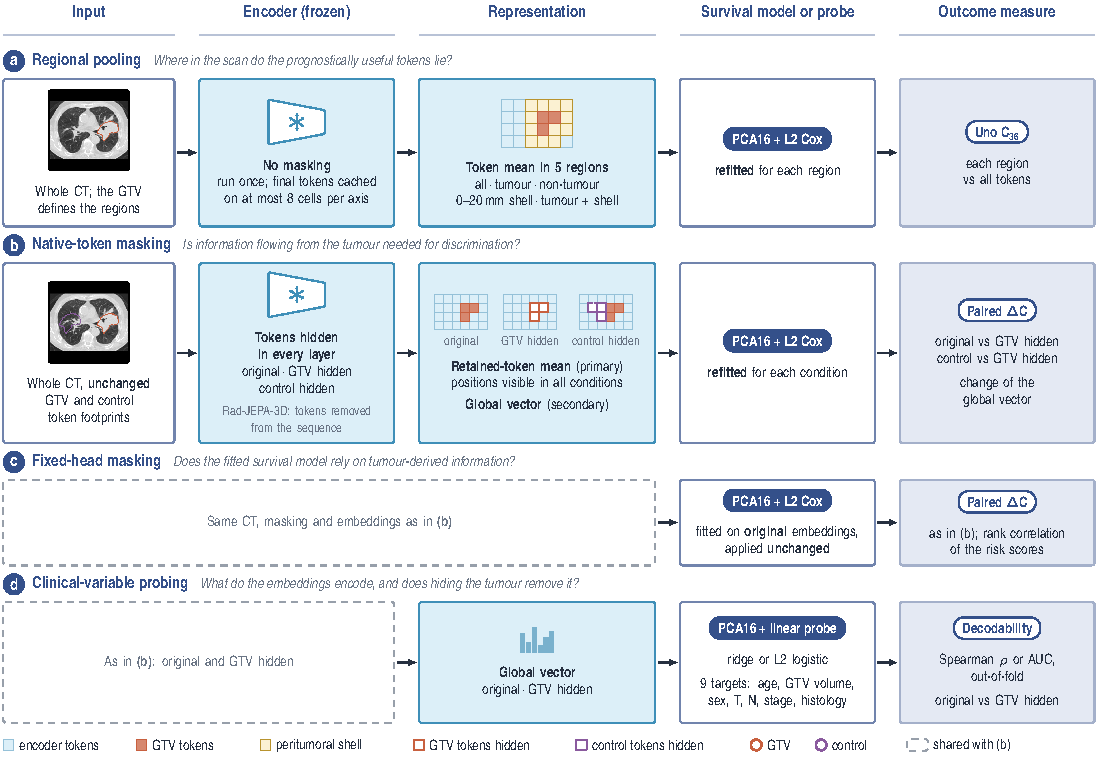
\includegraphics[width=\linewidth]{figures/rq3_design.pdf}
\caption{Design of the four tumour-dependence analyses (RQ3). Each row shows the input, the frozen encoder, the representation, the survival model or probe and the outcome measure. All survival models and probes were fitted on the development folds, with penalties selected by three-fold inner cross-validation, and evaluated on the same five outer test folds. (a) Regional pooling pools the cached final tokens of the unmasked encoder over regions defined by the primary tumour (GTV). (b) Native-token masking leaves the CT unchanged and hides, in every layer of the encoder, the native tokens that contain a GTV voxel, or the same number of tokens around the GTV shape translated within the same axial level (control). Each CT is encoded three times: original, GTV hidden and control hidden. In all three, the primary representation averages the tokens at the same positions, outside both the GTV and the control region, so the conditions differ only in what these tokens received from the hidden region inside the encoder. (c) Fixed-head masking uses the embeddings of (b) but does not refit the survival model. (d) Probing decodes clinical variables from the global vector, with and without the tumour hidden. The CT slice (LUNG1-001) and the control outline are illustrative; grid icons show a single axial level, whereas pooling and masking were applied to the three-dimensional token grid.}
\label{fig:rq3design}
\end{figure}


\paragraph{Regional pooling analysis.} The cached final tokens of each encoder were pooled over five regions defined from the GTV, without re-encoding the CT: all tokens; tumour tokens, weighted by the fraction of each token occupied by the GTV; non-tumour tokens with no GTV overlap; a peritumoral shell from 0 to 20 mm around the GTV; and the union of tumour and shell (Figure~\ref{fig:rq3design}a). Each pooled vector was passed to the frozen head. Because the tokens had already exchanged information inside the encoder, the non-tumour pool still contains information that came from the tumour; this analysis therefore asks \emph{where} useful token positions lie, not whether the tumour is needed.

\paragraph{Native-token masking analysis.} To remove the tumour's contribution inside the encoder, every native token containing a GTV voxel was hidden in every layer of the frozen encoder, while the CT input was left unchanged (Figure~\ref{fig:rq3design}b). In attention-based encoders, the keys of the hidden tokens were masked in every attention layer, and their outputs were excluded from every pooling; for a transformer this is equivalent to removing the tokens while keeping the positions of the others. In CT-CLIP, attention is not the only route between tokens: its blocks also mix neighbouring tokens through depthwise convolutions, so the hidden tokens were additionally set to zero at the input of every such convolution. Rad-JEPA-3D is a state-space hybrid without attention to mask, so the hidden tokens were removed from the sequence through the encoder's own context-index mechanism used during its pretraining. A leakage test replaced the hidden voxels with random noise: with masking on, the retained tokens and global vectors did not change for any encoder.

A loss of discrimination after hiding the GTV would not, on its own, show that the tumour matters, because hiding any region of the scan changes the representation, even a region with no prognostic information. To separate the effect of hiding the tumour from the effect of hiding tokens as such, we added a control condition, which hid the same number of tokens around the GTV shape translated to another position at the same axial level. The contrast between the control-hidden and tumour-hidden conditions therefore isolates the contribution of the tumour; a valid control was available for 403 patients. The primary pooling was the mean of the tokens visible in every condition, so that the original, tumour-hidden and control-hidden conditions were pooled over identical positions and differed only in whether those tokens could receive information from the hidden region. The encoder's own global vector was a secondary representation. Each condition was passed to a frozen head refitted for that condition. The analysis also measured how much the global vector changed relative to the original, to separate a change in the representation from a change in discrimination.

\paragraph{Fixed-head masking analysis.} Refitting the head on masked embeddings lets it adapt to the perturbation. In this analysis, the frozen head fitted on the original embeddings was applied unchanged to the tumour-hidden and control-hidden embeddings, which asks whether the fitted model relies on tumour-derived information.

\paragraph{Clinical-variable probing.} To describe what the embeddings encode, we tested how well clinical variables could be decoded from the global vectors, in the original and tumour-hidden conditions. The targets were age and log GTV volume (Spearman correlation) and male sex, T3--T4, any nodal involvement, N2--N3, stage III, squamous histology and adenocarcinoma (area under the ROC curve). Probes were ridge or L2-regularized logistic regressions on PCA16, with the penalty chosen by three-fold inner cross-validation; they were evaluated on the pooled out-of-fold predictions of the same outer folds, and all components were also used as a sensitivity analysis. Decodability shows that a variable is encoded; it does not show that the survival prediction uses it.

\subsubsection{RQ4: external evaluation}\label{sec:external}
RQ4 asks whether discrimination, incremental clinical value and calibration transfer to an external cohort, that is, whether models developed on LUNG1 keep their performance when applied, without any change, to patients from other institutions. Two analyses address it: the \emph{external evaluation} applies the models of RQ1 to NSCLC-Radiogenomics; the \emph{external LoRA analysis}, added as exploratory, does the same for the adapted encoders of RQ2.

For the \emph{external evaluation}, 22 models were refitted on all 416 LUNG1 patients with the same selection procedure used internally (penalties by three-fold cross-validation on the 416 patients; imputation, scaling and dimensionality reduction fitted on them): the nested clinical models, \model{Stage+Volume}, the radiomic model, the frozen head of every representation, and the Hosny zero-shot score. The external CTs received exactly the same preprocessing as LUNG1, without harmonization of intensities, kernels or slice thickness, because the aim was to test the models as they would be applied to a new hospital. The only correction was a decoding one: out-of-field padding stored below $-1024$ HU by some scanners was set to $-1024$ HU, the minimum value in every LUNG1 scan. No external recalibration was applied.

The four primary contrasts, fixed in advance, were COLIPRI vs \model{Stage+Volume}, \model{Clinical+Volume+COLIPRI} vs \model{Clinical+Volume}, COLIPRI vs the Pai lesion encoder, and COLIPRI vs Hosny zero-shot. Secondary outcomes were the concordance of all other models, the concordance at 60 months, the calibration of absolute risk and the Spearman correlation between internal and external concordance across models, which asks whether the ranking of pipelines transports. The trainable heads and the adaptation models were not carried over to the original external evaluation, because none of them had exceeded the frozen head internally at the time the external protocol was fixed.

In the \emph{external LoRA analysis}, LoRA models for all five encoders were trained on all 416 LUNG1 patients with the fixed adaptation configuration, frozen in the same way and evaluated on the external cohort, with paired comparisons against the corresponding frozen heads. This analysis was added after the external cohort had been examined in the original evaluation and uses a configuration chosen on LUNG1 test folds.

\subsection{Performance measures and statistical analysis}\label{sec:stats}
\paragraph{Discrimination.} The primary measure was Uno's concordance index truncated at 36 months (Uno C),\cite{uno2011} which weights comparable pairs by the inverse probability of censoring and is therefore less dependent on the censoring distribution than Harrell's index. For test patients with observed time $T_i$, event indicator $\delta_i$ and predicted risk $\eta_i$,
\begin{equation}\label{eq:unoc}
C_\tau=\frac{\sum_{i}\sum_{j}\delta_i\,\hat{G}(T_i)^{-2}\,\mathbf{1}(T_i<T_j,\;T_i\le\tau)\left[\mathbf{1}(\eta_i>\eta_j)+\frac{1}{2}\mathbf{1}(\eta_i=\eta_j)\right]}{\sum_{i}\sum_{j}\delta_i\,\hat{G}(T_i)^{-2}\,\mathbf{1}(T_i<T_j,\;T_i\le\tau)},
\end{equation}
where $\hat{G}$ is the Kaplan--Meier estimate of the censoring survival function, $\tau=36$ months, and ties in predicted risk count as one half. Internally, the censoring distribution was estimated from the development patients of each outer fold, and the primary estimate was the mean of the five test-fold values. Externally, the censoring distribution was estimated from the relevant external population.

\paragraph{Calibration.} Absolute risk was assessed externally by comparing observed mortality at 36 months (Kaplan--Meier) with mean predicted mortality, using the LUNG1 Breslow baseline hazard, and by the calibration slope, the coefficient of a Cox regression of the outcome on the linear predictor.\cite{vancalster2019,austin2020}

\paragraph{Uncertainty and tests.} Uncertainty was estimated with paired patient bootstrap resampling. Internally, test patients were resampled within each fixed fold and the fold estimates were averaged, with the same resamples shared by all models compared; externally, patients were resampled from the external population. We used 1,000 resamples for the clinical increment and trainable-model comparisons, 300 for the masking analyses and 2,000 for the external evaluation. Intervals are 95\% percentile intervals, and $p$ values come from a two-sided Wald test with the bootstrap standard error. These intervals condition on the fitted models and on the fold assignment; they do not include the variability from refitting the models on different patients.

Because most analyses involved several comparisons, $p$ values were adjusted with the Holm method within families of comparisons fixed in advance. Each of the following formed one family: the five primary contrasts of the clinical increment analysis (Section~\ref{sec:frozen}); each of its secondary contrasts, repeated across encoders (image over \model{Clinical+Volume}, clinical over image, radiomics over image, and image vs radiomics); the 22 comparisons of a trainable model with the frozen head of the same encoder (seven multilayer perceptron, five survival query adapter, five LoRA and five partial fine-tuning models; Section~\ref{sec:selected}); the four primary contrasts of the external evaluation (Section~\ref{sec:external}); and the comparisons of each external model with chance. Intervals for the masking and probing analyses (Section~\ref{sec:perturbation}), the label-budget analysis (Section~\ref{sec:selected}) and the external LoRA analysis (Section~\ref{sec:external}) are reported without multiplicity adjustment, and no hypothesis test is attached to the preliminary fixed-epoch analysis. A nonsignificant difference was not interpreted as absence of a difference: equivalence was declared when the 90\% bootstrap interval of a difference lay within a margin of $\pm0.03$ Uno C, fixed in advance (two one-sided tests), and for every contrast we report the minimum detectable difference, $(z_{0.975}+z_{0.80})$ times the bootstrap standard error. Contrasts smaller than this value are reported as inconclusive rather than negative.

\subsection{Implementation}
Survival models were implemented in Python with PyTorch Lightning for the neural models and lifelines for the linear Cox models; radiomic features were extracted with PyRadiomics 3.0.1. Neural models optimized the Cox partial likelihood with Efron ties, with the risk-set computations in single precision. Internal training used BF16 mixed precision on NVIDIA A100 GPUs; the external LoRA models were trained with FP16 mixed precision on an NVIDIA V100 for COLIPRI and TANGERINE and with BF16 on an A100 for the other three encoders. Each run stored a protocol file with the hashes of the cohort, the fold assignment, the encoder checkpoint and the cached inputs.
\gap{Add the code repository URL and the full list of software versions after the release inventory is verified.}
